\documentclass{../notatki}
\usepackage{float}

\title{Języki formalne}

\begin{document}

\tableofcontents

\newpage

\section{Literatura}

\begin{itemize}
  \item J.E. Hopencroft "Wprowadzenie do teorii automatów i obliczeń"
  \item M. Sipser "Wprowadzenie do teorii obliczeń"
  \item G.E. Revesz "Introduction to formal languages"
  \item H.R. Lewin, Papadimitriou "Elements of the Theory of Computation"
\end{itemize}

\section{Język}

$$
\infty \text{ zdań} + n \text{ reguł} = \text{język}
$$

\subsection{Funkcje języka}

\begin{enumerate}
  \item Poznawcza
  \item Społeczna
  \item Ekspresywna
\end{enumerate}

\subsection{Nauka o języku}

\begin{enumerate}
  \item syntaktyka - budowa
  \item semantyka - co znaczy?
  \item pragmatyka - jak się używa?
\end{enumerate}
Przykład:$2 + 3 \cdot 4$: różna semantyka $\rightarrow$
wieloznaczność syntaktyczna

\subsection{Definicja}

Język składa się z gramatyk i automatów. Gramatyka generuje język,
automat rozpoznaje język.

\begin{figure}[H]
  \centering
  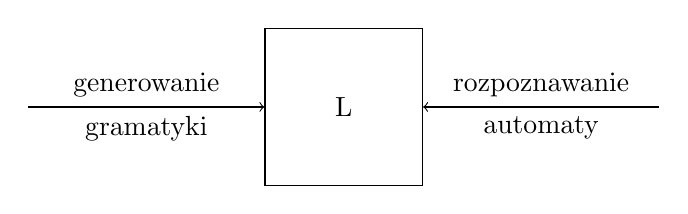
\begin{tikzpicture}[node distance=2cm]
    \node[draw, minimum size=2cm] (square) {L};
    \draw[<-] (square.west) -- node[anchor=south]{generowanie}
    node[anchor=north]{gramatyki} ++(-3,0);
    \draw[<-] (square.east) -- node[anchor=south]{rozpoznawanie}
    node[anchor=north]{automaty} ++(3,0);
  \end{tikzpicture}
  \caption{Ilustracja relacji języków, automatów i gramatyk}
\end{figure}

\section{Alfabet}

Alfabet to zbiór atomowych dozwolonych symboli. Przykład: $\{a, b, c, d\}$

\section{Słowo}

Słowo to skończony ciąg symboli nad alfabetem.

\begin{itemize}
  \item $\varepsilon$ - słowo puste
  \item $\{K, L, O, P, S\} \ne "KLOPS"$, ponieważ słowa mają dodane
    znaczenie, w postaci tego do którego języka należą.
\end{itemize}

\subsection{Konkatenacja}

\begin{itemize}
  \item $\text{Dla } P=a_1...a_n \text{ i } Q=b_1...b_n, \text{ to }
    PQ=a_1...a_nb_1...b_n$
  \item $P\epsilon = P$
  \item $\epsilon\epsilon = \epsilon$
\end{itemize}

\subsection{Podsłowo}

\begin{itemize}
  \item $P = Q_1 | Q | Q_2$
  \item $Q \subset P$
\end{itemize}

\subsection{Długość słowa}

\begin{itemize}
  \item $|\epsilon| = 0$
  \item $|Pa| = |P| + 1$
  \item $|PQ| = |P| + |Q|$
\end{itemize}

\subsection{Potęga słowa}

\begin{itemize}
  \item $P^0 = \epsilon$
  \item $P^{n + 1} = P^nP$
\end{itemize}

\subsection{Odbicie}

\begin{itemize}
  \item $\epsilon^-1 = \epsilon$
  \item $(Pa)^-1 = aP^-1$
\end{itemize}

\section{Język}

Zbiór dozwolonych słów nad alfabetem.

\begin{itemize}
  \item $V^*$ - zbiór wszystkich języków
  \item $V^+ = V^* \{\epsilon\}$
  \item $L \in V^*$
  \item $\{a, ab\} \ne \{\epsilon, a, ab\}$ ponieważ inaczej operacje
    na językach by nie działały
\end{itemize}

\subsection{Konkatenacja języków}

$$
L_1 = \{a, aa\}, L_2 = \{b, aba\}, L_1L_2 = \{ab, aaba, aab, aaaba\}
$$

\begin{table}[H]
  \centering
  \begin{tabular}{c|c|c}
    \backslashbox{$L_2$}{$L_1$} & a    & aa \\ \hline
    b   & ab   & aab \\
    aba & aaba & $aaaba$ \\
  \end{tabular}
  \caption{Tabela konkatenacji języków $L_1$ i $L_2$}
\end{table}

$|L_1L_2| \le |L_1| \cdot |L_2|$ bo eps wszystko psuje

$$
L_1 = \{a^n : n \ge 0\}, L_2 = \{b^n : n \ge 0\}, L_1L_2 = \{a^nb^m :
n, m \ge 0\}
$$

\subsection{Potęga języka}

$$
L = \{a, ab\}, L^0 = \{\epsilon\}, L^1 = \{a, ab\}, L^2 = L \cdot L
$$
\textbf{Potęgowanie na językach jest dziwne}

$$
L = \{a^n : n \ge 0\}, L^2 = \{a^n a^m : a, m \ge 0\} = \{a^n : a \ge 0\} = L
$$
Potęgowanie języku \textbf{nie} zwiększyło mocy
$$
L = \{a^n : n > 0\}, L^2 = \{a^n a^m : a, m > 0\} = L \setminus \{a\}
= \{a^n : n > 1\}
$$
Potęgowanie języku \textbf{zmniejszyło} moc

\subsection{Odbicie języka}

$$
L^{-1} = \{P^{-1} : P \in L\}
$$

\subsection{Dzielenie słów}

$$
P \in L^n \rightarrow \text{ można podzielić } P \text{ na } n \text{
(niekoniecznie różnych) słów}
$$

$$
L = \{a, ab\}, "aababaabab" \in L^n, n=?
$$
Jest to problem wykładniczy, który wymaga stworzenia drzewa różnych możliwości.

\section{Domknięcie Kleenego}

$$
L^* = \bigcup_{n \ge 0}^{\infty}L^n
$$

$$
L^+ = \bigcup_{n \ge 1}^{\infty}L^n
$$

$$
L_1 = \{a\}, L_1^* = \{a^n : n \ge 0\}, L_1^+ = \{a^n : n > 0\}
$$

$$
L_2 = \{\epsilon, a\}, L_2^* = \{a^n : n \ge 0\} = L_2^+
$$

$$
L = \{aa, ab, ba, bb\}, L^* = \{P \in \{a, b\}^* : 2 | |P|\} =
\text{wszystkie słowa nad alfabetem {a, b} o parzystej długości}
$$

\begin{itemize}
  \item $L^+ \subset L^*$
  \item $\epsilon \in L \rightarrow L^+ = L^*$
  \item $(L^*)^* = L^*$
  \item $L_1 \subset L_2 \rightarrow L_1^* \subset L_2^*$
\end{itemize}

$$
L = \{a^n : n > 1\}, L^1 \ne L^2, L^* = L
$$

\section{Automaty Regularne}

\begin{itemize}
  \item nieskończona taśma
  \item rejestry
  \item w każdym rejestrze symbol z alfabetu T
  \item głowica, która porusza się od lewej do prawej po rejestrach
    taśmy, aż do momentu, kiedy napotka pusty rejestr. Głowica zawsze
    jest w jednym ze stanów z zbioru stanów
\end{itemize}

\subsection{Deterministyczne automaty skończone}

Automat skończenie stanowy jest uporządkowaną piątką
$$
\mathfrak{A} = \langle K,T,\delta,q_0,H \rangle
$$

\begin{itemize}
  \item $K$   zbiór stanów
  \item $T$   alfabet - symbole z tego alfabetu znajdują się w rejestrach
  \item $\delta: K \times T \rightarrow K$  funkcja przejścia automatu
  \item $q_0$ stan początkowy automatu
  \item $H$ zbiór stanów akceptowalnych/końcowych
\end{itemize}

\subsubsection{Funkcja przejść}

Zbiory $K$ i $T$ są skończone, co oznacza, że funkcję $\delta$ można
przedstawić w formie tabelki. Przykład:

$$
K = \{q_0, q_1, q_2\}, T = \{a,b\}, H = \{q_2\}
$$

$$
\delta: K \times T \rightarrow K
$$

\begin{figure}[H]
  \centering
  \resizebox{0.5\textwidth}{!}{
    \begin{minipage}{0.25\textwidth}
      \begin{tabular}{c|c|c}
        \backslashbox{$K$}{$T$} & a    & b \\ \hline
        $\rightarrow q_0$ & $q_2$ & $q_1$ \\
        $q_1$             & $q_0$ & $q_1$ \\
        $\underline{q_2}$ & $q_1$ & $q_2$ \\
      \end{tabular}
    \end{minipage}
    \begin{minipage}{0.25\textwidth}
      \begin{tikzpicture}[shorten >=1pt,node distance=2cm,on grid,auto]
        \node[state,initial] (q_0)   {$q_0$};
        \node[state] (q_1) [below right=of q_0] {$q_1$};
        \node[state,accepting] (q_2) [above right=of q_0] {$q_2$};
        \path[->]
        (q_0) edge [bend left] node {a} (q_2)
        edge [bend left] node {b} (q_1)
        (q_1) edge [loop right] node {b} ()
        edge [bend left] node {a} (q_0)
        (q_2) edge [loop right] node {b} ()
        edge [bend left] node {a} (q_1);
      \end{tikzpicture}
    \end{minipage}
  }
  \caption{Tabela konkatenacji języków $L_1$ i $L_2$ oraz graf przejść automatu}
  \label{fig:automat:example}
\end{figure}

\subsubsection{Rozszerzona funkcja przejść}

$$
\stackrel{\wedge}{\delta}: K \times T^* \rightarrow K
$$

\begin{itemize}
  \item $\stackrel{\wedge}{\delta}(q, \epsilon) = q$
  \item $\stackrel{\wedge}{\delta}(q, Pa) =
    \delta(\stackrel{\wedge}{\delta}(q, P), a)$
\end{itemize}

$$
L(\mathfrak{A}) = \{P \in T^* : \stackrel{\wedge}{\delta}(q_0, P) \in H\}
$$

\subsubsection{Przykład}

Narysuj diagram przejścia deterministycznego automatu skończenie
stanowego $\mathfrak{A}$ w którym $T=\{0, 1\}, P \in L(\mathfrak{A})$
wtedy i tylko wtedy gdy w $P$ występuje na pierwszym od końca miejscu.

\begin{figure}[H]
  \centering
  \begin{tikzpicture}[shorten >=1pt,node distance=2cm,on grid,auto]
    \node[state,initial] (q_0)   {$q_0$};
    \node[state,accepting](q_1) [right=of q_0] {$q_1$};
    \path[->]
    (q_0) edge [bend left] node {1} (q_1)
    edge [loop above] node {0} ()
    (q_1) edge [bend left] node {0} (q_0)
    edge [loop below] node {1} ();
  \end{tikzpicture}
  \caption{Diagram przejścia automatu do wykrywania 1 na pierwszym
  miejscu od końca}
  \label{fig:automat:1end}
\end{figure}

Narysuj diagram przejścia deterministycznego automatu skończenie
stanowego $\mathfrak{A}$ w którym $T=\{0, 1\}, P \in L(\mathfrak{A})$
wtedy i tylko wtedy gdy w $P$ występuje na drugim od końca miejscu 1.

\begin{figure}[H]
  \centering
  \begin{tikzpicture}[shorten >=1pt,node distance=2.0cm,on grid,auto]
    \node[state,initial] (q_0)   {$q_0$};
    \node[state](q_1) [right=of q_0] {$q_1$};
    \node[state,accepting](q_2) [above right=of q_1] {$q_2$};
    \node[state,accepting](q_3) [below right=of q_1] {$q_3$};
    \path[->]
    (q_0) edge   node {1} (q_1)
    edge  [loop above] node {0} ()
    (q_1) edge  [bend left] node {0} (q_3)
    edge  [bend left] node {1} (q_2)
    (q_2) edge  [loop above] node {1} ()
    edge  [bend left] node {0} (q_3)
    (q_3) edge  [bend left] node {1} (q_1)
    edge  [bend left] node {0} (q_0);
  \end{tikzpicture}
  \caption{Diagram przejścia automatu do wykrywania 1 na drugim
  miejscu od końca}
  \label{fig:automat:2end}
\end{figure}

Widać na diagramie \ref{fig:automat:2end} wprost zależność że w
zależności od miejsca od końca na którym ma być jeden rośnie ilość stanów.
Ilość stanów maszyny $|K|$ do wykrywania 1 na $n$-tym miejscu od
końca można wyrazić w następujący sposób: $|K| = 2^n$

\subsection{Niedeterministyczne automaty skończone}

\begin{itemize}
  \item zamiast jednego stanu początkowego jest zbiór stanów początkowych
  \item niedeterministyczna funkcja przejścia, która zwraca zbiór
    wyjściowych stanów
\end{itemize}

$$
\mathfrak{A} = \langle K,T,\delta,Q_0,H \rangle
$$
gdzie oznaczenia są identyczne jak dla deterministycznego automatu z
dwoma różnicami:

\begin{itemize}
  \item $\delta: K \times T \rightarrow a \in K$  funkcja przejścia automatu
  \item $Q_0$ zbiór stanów początkowych automatu
\end{itemize}

\begin{figure}[H]
  \centering
  \begin{tikzpicture}[shorten >=1pt,node distance=2cm,on grid,auto]
    \node[state,initial] (q_0)   {$q_0$};
    \node[state](q_1) [right=of q_0] {$q_1$};
    \node[state,accepting](q_2) [right=of q_1] {$q_2$};
    \path[->]
    (q_0) edge  node {1} (q_1)
    edge  [loop above] node {0,1} ()
    (q_1) edge  node {0,1} (q_2);
  \end{tikzpicture}
  \caption{Niedeterministyczna wersja automatu $\mathfrak{A}$ z
  rysunku \ref{fig:automat:2end}}
  \label{fig:automat:2end-ndet}
\end{figure}

Jak widać zamiast 4 stanów potrzeba tylko 3, to dlatego, że dla
wersji niedeterministycznej $|K| = n + 1$

\subsubsection{Rozszerzona funkcja przejść}

$$
\stackrel{\wedge}{\delta}: P(K) \times T^* \rightarrow P(K)
$$

\begin{itemize}
  \item $\stackrel{\wedge}{\delta}(A, \epsilon) = A$
  \item $\stackrel{\wedge}{\delta}(A, Pa) = \bigcup_{q \in
    \stackrel{\wedge}{\delta}(A, P)}\delta(q, a)$
\end{itemize}

$$
\stackrel{\wedge}{\delta}(\{p\}, a) = \delta(p, a)
$$

$$
L(\mathfrak{A}) = \{P \in T^* : \stackrel{\wedge}{\delta}(Q_0, P)
\cap H \ne \emptyset\}
$$

\subsubsection{Twierdzenie Scotta}

\begin{itemize}
  \item każdy \textbf{nie}deterministyczny automat skończony można
    zastąpić równoważnym deterministycznym automatem skończonym
    $$\mathfrak{L}_{ndet} \subset \mathfrak{L}_{det}$$
  \item każdy deterministyczny automat skończony można zastąpić
    równoważnym \textbf{nie}deterministycznym automatem skończonym
    $$\mathfrak{L}_{det} \subset \mathfrak{L}_{ndet}$$
  \item liczba stanów automatu deterministycznego jest wykładnicza w
    stosunku do liczby stanów automatu niedeterministycznego
\end{itemize}

$$\mathfrak{L}_{det} = \mathfrak{L}_{ndet}$$
Zatem co nam daje niedeterministyczność? Przede wszystkim prostotę,
ale kosztem wykładniczej złożoności.

Narysuj diagram przejścia deterministycznego automatu skończenie
stanowego $\mathfrak{A}$ w którym $T=\{a\}, P \in L(\mathfrak{A})$
wtedy i tylko wtedy gdy $(2 | |P|) \vee (3 | |P|)$.

\begin{figure}[H]
  \centering
  \begin{tikzpicture}[shorten >=1pt,node distance=2cm,on grid,auto]
    \node[state,initial,accepting] (q_0)   {$q_0$};
    \node[state](q_1) [above right=of q_0] {$q_1$};
    \node[state, accepting](q_2) [right=of q_1] {$q_2$};
    \node[state, accepting](q_3) [below right=of q_2] {$q_3$};
    \node[state,accepting](q_4) [below left=of q_3] {$q_4$};
    \node[state](q_5) [left=of q_4] {$q_5$};
    \path[->]
    (q_0) edge  node {a} (q_1)
    (q_1) edge  node {a} (q_2)
    (q_2) edge  node {a} (q_3)
    (q_3) edge  node {a} (q_4)
    (q_4) edge  node {a} (q_5)
    (q_5) edge  node {a} (q_0);
  \end{tikzpicture}
  \caption{Diagram przejścia automatu do wykrywania słów o długości
  podzielnej przez 2 lub 3}
  \label{fig:automat:2or3}
\end{figure}

Jak widzimy na diagramie \ref{fig:automat:2or3} przyjmuje postać
cyklu o okresie 6, ponieważ $NWW(3,2)=6$.
Problem z diagramami deterministycznym się pojawia dla wyższych
liczb, np.: $7$ i $5$, wtedy $NWW(7,5)=35$.
Zatem narysujmy diagram niedeterministyczny \ref{fig:automat:5or7}.

\begin{figure}[H]
  \centering
  \begin{tikzpicture}[shorten >=1pt,node distance=2cm,on grid,auto]
    \node[] (initial) {start};
    \node[state, accepting] (q5_0) [left=of initial] {$q_0^5$};
    \node[state] (q5_1) [below left=of q5_0] {$q_1^5$};
    \node[state] (q5_2) [left=of q5_1] {$q_2^5$};
    \node[state] (q5_4) [above left=of q5_0] {$q_4^5$};
    \node[state] (q5_3) [left=of q5_4] {$q_3^5$};

    \node[state, accepting] (q7_0) [right=of initial] {$q_0^7$};
    \node[state] (q7_1) [above right=of q7_0] {$q_1^7$};
    \node[state] (q7_2) [right=of q7_1] {$q_2^7$};
    \node[state] (q7_3) [right=of q7_2] {$q_3^7$};
    \node[state] (q7_6) [below right=of q7_0] {$q_6^7$};
    \node[state] (q7_5) [right=of q7_6] {$q_5^7$};
    \node[state] (q7_4) [right=of q7_5] {$q_4^7$};

    \path[->]
    (q5_0) edge node {a} (q5_1)
    (q5_1) edge node {a} (q5_2)
    (q5_2) edge node {a} (q5_3)
    (q5_3) edge node {a} (q5_4)
    (q5_4) edge node {a} (q5_0);

    \path[->]
    (q7_0) edge node {a} (q7_1)
    (q7_1) edge node {a} (q7_2)
    (q7_2) edge node {a} (q7_3)
    (q7_3) edge node {a} (q7_4)
    (q7_4) edge node {a} (q7_5)
    (q7_5) edge node {a} (q7_6)
    (q7_6) edge node {a} (q7_0);

    \draw[->] (initial) -- (q5_0);
    \draw[->] (initial) -- (q7_0);
  \end{tikzpicture}
  \caption{Diagram przejścia automatu ndet do wykrywania słów o
  długości podzielnej przez 5 lub 7}
  \label{fig:automat:5or7}
\end{figure}

Jako, że automaty niedetermnistyczne pozwalają na kilka stanów
początkowych, to tworzymy diagram niespójny, który w zależności od
tego czy $|P|$ jest podzielne przez $5$ czy $7$ przechodzi do
odpowiedniego pod-automatu.
Najłatwiej to można sobie wyobrazić jako dwa równoległe automaty z
alternatywą na koniec.

\subsubsection{Przekształcenie niedet \texorpdfstring{$\rightarrow$}{->} det}

$$
\mathfrak{A} = \langle K,T,\delta,Q_0,H \rangle
$$

$$
\mathfrak{A}' = \langle K',T',\delta',q_0',H' \rangle
$$

$$
L(\mathfrak{A}) = L(\mathfrak{A}')
$$

\begin{itemize}
  \item $T' = T$ bo nie ma sensu zmieniać taśmy
  \item $K' = P(K)$ \textbf{Wykładniczy wzrost liczby stanów}\\
    w przekształceniu będziemy używać systemu etykiet(konstrukcja
    potęgowa) aby zamieniać zbiory stanów na pojedyncze stany
    $$
    \{q_0,q_1\} = q^{01}
    $$
    $$
    P(K) = \{q^\emptyset, q^1, q^0, q^{10}, ...\}
    $$
  \item $q_0' = Q_0$ - stan odpowiadający zbiorowi stanów początkowych
  \item $H' = \{A \in K' : A \cap H \ne \emptyset\}$
  \item $\delta'(A, a) = \bigcup_{q \in A}\delta(q, a)$
\end{itemize}
Dla automatu \ref{fig:automat:2end-ndet} zbudujmy równoważny automat
deterministyczny.
Korzystając z powyższych zasad otrzymujemy:

\begin{itemize}
  \item $K' = P(K) = \{\emptyset, \{q_0\}, ..., \{q_1, q_2\}, \{q_0,
    q_1, q_2\}\} = \{q^\emptyset, q^0, ..., q^{12}, q^{012}\}$
  \item $H' = \{q^2, q^{12}, q^{02}, q^{012}\}$
  \item $q_0' = \{q_0\} = q^0$
\end{itemize}

\begin{figure}[H]
  \centering
  \resizebox{0.5\textwidth}{!}{

    \begin{minipage}{0.25\textwidth}
      \begin{tabular}{c|c|c}
        \backslashbox{$K'$}{$T$} & 0             & 1 \\ \hline
        $q^\emptyset$            & $q^\emptyset$ & $q^\emptyset$ \\
        $\rightarrow q^0$        & $q^0$         & $q^{01}$ \\
        $q^1$                    & $q^2$         & $q^2$ \\
        $\underline{q^2}$        & $q^\emptyset$ & $q^\emptyset$ \\
        $q^{01}$                 & $q^{02}$      & $q^{012}$ \\
        $\underline{q^{12}}$     & $q^2$         & $q^2$ \\
        $\underline{q^{02}}$     & $q^0$         & $q^{01}$ \\
        $\underline{q^{012}}$    & $q^{02}$      & $q^{012}$ \\
      \end{tabular}
    \end{minipage}
    \begin{minipage}{0.45\textwidth}
      \begin{tikzpicture}[shorten >=1pt,node distance=2cm,on grid,auto]
        \node[state,initial] (q_0)   {$q^0$};
        \node[state](q_1) [right=of q_0] {$q^{01}$};
        \node[state,accepting](q_2) [above right=of q_1] {$q^{012}$};
        \node[state,accepting](q_3) [below right=of q_1] {$q^{02}$};
        \node[state,accepting](q_4) [above right=of q_3] {$q^2$};
        \node[state](q_6) [right=of q_4] {$q^\emptyset$};
        \node[state](q_5) [above=of q_4] {$q^1$};
        \node[state,accepting](q_7) [below=of q_4] {$q^{12}$};
        \path[->]
        (q_0) edge   node {1} (q_1)
        edge  [loop above] node {0} ()
        (q_1) edge  [bend left] node {0} (q_3)
        edge  [bend left] node {1} (q_2)
        (q_2) edge  [loop above] node {1} ()
        edge  [bend left] node {0} (q_3)
        (q_3) edge  [bend left] node {1} (q_1)
        edge  [bend left] node {0} (q_0)
        (q_4) edge node {0, 1} (q_6)
        (q_5) edge node {0, 1} (q_4)
        (q_7) edge node {0, 1} (q_4)
        (q_6) edge [loop above] node {0, 1} (q_6);
      \end{tikzpicture}
    \end{minipage}
  }
  \caption{Zdeterminizowany automat z rysunku
  \ref{fig:automat:2end-ndet} i jego tabela przejść}
  \label{fig:automat:2end-det}
\end{figure}

Jak widać na diagramie \ref{fig:automat:2end-det} liczba stanów
wzrosła z 3 do 8, co jest zgodne z przewidywaniami.
Jednocześnie widać, że diagram \ref{fig:automat:2end} zawiera się w
diagramie \ref{fig:automat:2end-det}, co niekoniecznie oznacza, że są
sobie równoważne, lecz jako, że stany dodatkowe są nieosiągalne to te
dwa automaty są równoważne.
\textbf{Nie zawsze równoważność automatów będzie tak oczywista.}

\subsection{Automaty z przejściem}

Co jeśli moglibyśmy zmienić stan ale nie ruszyć głowicy? Wtedy mamy
do czynienia z automatem z przejściem.

$$
\epsilon \in T, \epsilon = \text{nie ruszaj głowicy automatu}
$$

$$
\delta: K \times (T \cup \{\epsilon\}) \rightarrow P(K)
$$

\textbf{Każdy automat z przejściem jest niedeterministyczny}

\begin{figure}[H]
  \centering
  \begin{tikzpicture}[shorten >=1pt,node distance=2cm,on grid,auto]
    \node[state,initial] (q_0)   {$q_0$};
    \node[state](q_1) [right=of q_0] {$q_1$};
    \node[state,accepting](q_2) [right=of q_1] {$q_2$};
    \path[->]
    (q_0) edge  node {$\epsilon$} (q_1)
    edge  [loop above] node {0} ()
    (q_1) edge  node {$\epsilon$} (q_2)
    edge  [loop above] node {1} ();
  \end{tikzpicture}
  \caption{Automat z przejściem}
  \label{fig:automat:epsilon}
\end{figure}
Automat przedstawiony na rysunku \ref{fig:automat:epsilon} akceptuje
języki o następującej postaci $L(\mathfrak{A})=\{0^n1^m2^k: n,m,k \ge 0\}$.

\textbf{Nie istnieją różne epsilony:} $00\epsilon1\epsilon222 = 00122$

\subsubsection{Domknięcie stanu}

$$
E(q) = \text{zbiór stanów osiągalnych z } q \text{ przez dowolną
liczbę epsilonów}
$$

\begin{enumerate}
  \item $q \in E(q)$
  \item $r \in E(q) \wedge p \in \delta(r, \epsilon) \rightarrow p \in E(q)$
\end{enumerate}

\subsubsection{Domknięcie zbioru stanów}

$$
E(A) = \bigcup_{q \in A}E(q)
$$

\subsubsection{Rozszerzona funkcja przejść}

$$
\stackrel{\wedge}{\delta}: P(K) \times T^* \rightarrow P(K)
$$

\begin{itemize}
  \item $\stackrel{\wedge}{\delta}(A, \epsilon) = E(A)$
  \item $\stackrel{\wedge}{\delta}(A, Pa) = \bigcup_{q \in
    \stackrel{\wedge}{\delta}(A, P)}E(\delta(q, a))$
\end{itemize}

\subsubsection{Przekształcenie \texorpdfstring{$\epsilon
\rightarrow$}{eps ->} ndet}

$$
\mathfrak{A}' = \langle K',T',\delta',Q_0',H' \rangle
$$

$$
T' = T, K' = K, H' = H, Q_0' = E(Q_0), \delta'(A, a) = E(\delta(q, a))
$$

$$
\mathfrak{L_{ndet} = \mathfrak{L_{\epsilon}} = \mathfrak{L_{det}}}
$$

\begin{figure}[H]
  \centering
  \begin{tabular}{c|c|c|c}
    $\delta_\epsilon$ & a              & b         & $\epsilon$ \\ \hline
    $\rightarrow q_0$ & $\emptyset$    & $\{q_1\}$ & $\{q_2\}$  \\
    $q_1$             & $\{q_1, q_2\}$ & $\{q_2\}$ & $\emptyset$ \\
    \underline{$q_2$} & $\{q_0\}$    & $\emptyset$ & $\emptyset$ \\
  \end{tabular}
  \textbf{$\Longrightarrow$}
  \begin{tabular}{c|c|c}
    $\delta_{ndet}$              & a                           & b
    \\ \hline
    $\rightarrow q_0$             & $E(\emptyset)=\emptyset$    & $\{q_1\}$   \\
    $q_1$                         & $\{q_1, q_2\}$              & $\{q_2\}$   \\
    $\rightarrow \underline{q_2}$ & $E(\{q_0\})=\{q_0, q_2\}$   & $\emptyset$ \\
  \end{tabular}
  \caption{Przekształcenie automatu z przejściem na niedeterministyczny}
  \label{fig:automat:eps2ndet}
\end{figure}

\section{Wyrażenia regularne}

$$
Reg(V) = \text{zbiór wyrażeń regularnych nad alfabetem } V
$$

\begin{itemize}
  \item $o \in Reg(V)$
  \item $e \in Reg(V)$
  \item $a \in V \rightarrow a \in Reg(V)$
  \item $u, v \in Reg(V) \rightarrow (u + v), (u \cdot v), (u^*) \in Reg(V)$
\end{itemize}

\subsection{Operacje}

\textbf{W kolejności od najwyższego priorytetu do najniższego}

\begin{enumerate}
  \item $P \in Reg(V) \rightarrow L(P) \ne \emptyset$
  \item $L(u^*) = (L(u))^*$
  \item $L(uv) = L(u) \cdot L(v)$
  \item $L(u + v) = L(u) \cup L(v)$
  \item $L(u) = \{u\}$
\end{enumerate}

\subsection{Przykłady}

$$
L(ba^*) = \{ba^n : n \ge 0\}
$$

$$
L(ba^*) = L(b)L(a^*) = \{b\} \cdot (L(a))^* = \{b\} \cdot \{a\}^* =
\{ba^n : n \ge 0\}
$$

$L((a + b)^*ab(a + b)^*)$ - wszystkie słowa nad alfabetem $\{a, b\}$
zaczynające się od a i kończące się b

\subsection{Tw. Kleenego}

$$
\forall_{v \in Reg(V)}L(v) \subset \mathfrak{L}_{det}
$$

Każdy język generowany przez wyrażenie regularne jest językiem
akceptowanym przez automat skończony.
Dowód opiera się na konstrukcji automatu $\epsilon$ odpowiadającego
operatorowi wyrażenia regularnego.

\subsubsection{\texorpdfstring{$w = u + v$}{w = u + v}}

$$
L(u + v) = L(u) \cup L(v)
$$
$$
L(u) = L(\mathfrak{A}_u), L(v) = L(\mathfrak{A}_v)
$$
$$
L(\mathfrak{A}) = L(\mathfrak{A}_u) \cup L(\mathfrak{A}_v)
$$

\begin{figure}[H]
  \centering
  \begin{tikzpicture}[shorten >=1pt,node distance=2cm,on grid,auto]
    \node[state,initial] (q_0)   {$q_0$};
    \node[rectangle, draw] (u) [above right=of q_0] {$\mathfrak{A}_u$};
    \node[rectangle, draw] (v) [below right=of q_0] {$\mathfrak{A}_v$};
    \path[->]
    (q_0) edge [bend left] node {$\epsilon$} (u)
    edge [bend right] node {$\epsilon$} (v);
  \end{tikzpicture}
  \caption{Konstrukcja automatu dla wyrażenia regularnego $u + v$}
  \label{fig:reg:plus}
\end{figure}

\subsubsection{\texorpdfstring{$w = uv$}{w = u}}

$$
L(uv) = L(u) \cdot L(v)
$$
$$
L(u) = L(\mathfrak{A}_u), L(v) = L(\mathfrak{A}_v)
$$
$$
L(\mathfrak{A}) = L(\mathfrak{A}_u) \cdot L(\mathfrak{A}_v)
$$

\begin{figure}[H]
  \centering
  \begin{tikzpicture}[shorten >=1pt,node distance=2cm,on grid,auto]
    \node[state,initial] (q_0)   {$q_0$};
    \node[rectangle, draw] (u) [right=of q_0] {$\mathfrak{A}_u$};
    \node[rectangle, draw] (v) [right=of u] {$\mathfrak{A}_v$};
    \path[->]
    (q_0) edge node {$\epsilon$} (u)
    (u) edge node {$\epsilon$} (v);
  \end{tikzpicture}
  \caption{Konstrukcja automatu dla wyrażenia regularnego $uv$}
  \label{fig:reg:concat}
\end{figure}

\subsubsection{\texorpdfstring{$w = u^*$}{w = u*}}

$$
L(u^*) = (L(u))^*
$$
$$
L(u) = L(\mathfrak{A}_u)
$$
$$
L(\mathfrak{A}) = (L(\mathfrak{A}_u))^*
$$

\begin{figure}[H]
  \centering
  \begin{tikzpicture}[shorten >=1pt,node distance=2cm,on grid,auto]
    \node[state,initial] (q_0)   {$q_0$};
    \node[rectangle, draw] (u) [right=of q_0] {$\mathfrak{A}_u$};
    \node[state,accepting] (q_1) [right=of u] {$q_1$};
    \path[->]
    (q_0) edge node {$\epsilon$} (u)
    (q_0) edge [bend right] node {$\epsilon$} (q_1)
    (u) edge node {$\epsilon$} (q_1)
    (u) edge [loop above] node {$\epsilon$} ();
  \end{tikzpicture}
  \caption{Konstrukcja automatu dla wyrażenia regularnego $u^*$}
  \label{fig:reg:star}
\end{figure}

\section{Klasy języków}

\begin{figure}[h]
  \centering
  \begin{tikzpicture}[shorten >=1pt,node distance=1cm,on
    grid,auto,rounded corners=0.5cm]
    \node[draw, circle] (reg) at (0,0) {$Reg$};
    \node[right=of reg] (cf) {$cf$};
    \node[fit=(reg) (cf), draw] (cfs) {};
    \node[left=of reg] (cs) {$cs$};
    \node[fit=(cfs) (cs), draw] (css) {};
    \node[below=of reg] (turing) {Rozpoznawane przez maszyny Turinga};
    \node[fit=(css) (turing), draw] (allturing) {};
  \end{tikzpicture}
  \caption{Nadzbiory języków regularnych}
  \label{fig:cls:reg}
\end{figure}

\subsection{Języki regularne}

\begin{figure}[H]
  \centering
  \begin{tikzpicture}[shorten >=1pt,node distance=2cm,on grid,auto]
    \node[state,initial] (q_0)   {$q_0$};
    \node[state,accepting] (q_1) [right=of q_0] {$q_1$};
    \node[state] (q_f) [right=of q_1] {$q_f$};
    \path[->]
    (q_0) edge [loop above] node {a} ()
    (q_0) edge node {b} (q_1)
    (q_1) edge [loop above] node {b} ()
    (q_1) edge node {b} (q_f)
    (q_f) edge [loop above] node {a,b} ();
  \end{tikzpicture}
  \caption{Konstrukcja automatu dla automatu $a^*b^*$}
  \label{fig:cls:ex1}
\end{figure}

Język regularny to język akceptowany przez wyrażenie regularne, czyli
język akceptowany przez automat skończony.

\begin{figure}[H]
  \centering
  \begin{tikzpicture}[shorten >=1pt,node distance=2cm,on grid,auto]
    \node[state,initial] (q_0)   {$q_0$};
    \node[state] (q_1) [right=of q_0] {$q_1$};
    \node[state,accepting] (q_2) [below=of q_1] {$q_2$};
    \node[state] (q_3) [right=of q_1] {$q_3$};
    \node[state] (q_4) [below=of q_3] {$q_4$};
    \node[state] (q_5) [right=of q_3] {$q_5$};
    \node[state] (q_6) [below=of q_5] {$q_6$};
    \path[->]
    (q_0) edge node {a} (q_1)
    (q_1) edge node {a} (q_3)
    (q_1) edge node {b} (q_2)
    (q_3) edge node {b} (q_4)
    (q_3) edge node {a} (q_5)
    (q_4) edge node {b} (q_2)
    (q_5) edge node {b} (q_6)
    (q_6) edge node {b} (q_4);
  \end{tikzpicture}
  \caption{Konstrukcja automatu akceptującego język $L = \{a^nb^n : 1
  \le n \le 3\}$ \textbf{bez śmietnika}}
  \label{fig:cls:ex2}
\end{figure}

\par \noindent \textbf{Czy można zapisać automat deterministyczny
(lub nie) skończenie stanowy, akceptujący język $L = \{a^nb^n : n \ge 1\}$ ?}

Nie da się, ponieważ wymagałoby to nieskończonej ilości stanów. Zatem
język $L$ nie jest językiem regularnym.

\subsubsection{Lemat o pompowaniu dla języków regularnych}

Służy do dowodzenia, że język \textbf{nie} jest regularny. \\
Jeżeli $L = L(\mathfrak{A})$\\to: istnieje $k \ge 0$, taki, że każde
słowo $P \in L$ o długości $|P| \ge k$ można zapisać jako $P = XYZ$,
spełniające warunki:\\
\begin{itemize}
  \item $Y \ne \epsilon$
  \item $|XY| \le k$
  \item $\forall_{i \ge 0} XY^iZ \in L$
\end{itemize}
Parafrazując: jeśli język jest regularny, to nie ma w nim słowa,
którego nie mógłbyś podzielić na trzy części, takie, że środkowa
część jest powtarzalna. \\

Lemat o pompowaniu jest warunkiem koniecznym ale nie wystarczającym.
To oznacza, że wszystkie języki regularne spełniają warunek lematu o
pompowaniu, ale nie wszystkie języki spełniający warunek lematu o
pompowaniu są regularne.
Warunkiem dostatecznym jest zdefiniowanie automatu skończenie
stanowego akceptującego język.

\textbf{Przykład zgodny} \\
Dlaczego język $L = \{a^nb^m : n,m \ge 1\}$ jest regularny?

\begin{itemize}
  \item $k > 2, P \in L$
  \item $|P| \ge k \rightarrow n + m \ge k$
  \item $P = a^{n - x}a^xb^m$ czyli $P = XYZ$ gdzie $X = a^{n - x}, Y
    = a^x, Z = b^m$
  \item $n - x + x < k \leftrightarrow |XY| \le k$
  \item dla $i \ge 0$ $XY^iZ = a^{n - x}a^{xi}b^m = a^{n + x(i -
    1)}b^m$, co jak widzimy jest w języku $L$
\end{itemize}
\textbf{Przykład niezgodny} \\
Dlaczego język $L = \{a^nb^n : n \ge 1\}$ nie jest regularny?

\begin{itemize}
  \item $k > 2, P \in L$
  \item $|P| \ge k \rightarrow 2n \ge k$
  \item $|XY| \le k \rightarrow XY = a^n \vee XY = b^n$
  \item dla $i = 2$ $XY^2Z = a^nb^nb^n \notin L$
\end{itemize}
\textbf{Zatem muszą istnieć języki nieregularne}

\subsubsection{Przechodniość regularności}

Z tw. Kleenego:

$$L_1,L_2 \in \mathfrak{L}_{reg} \rightarrow L_1 \cup L_2, L_1 \cdot
L_2, L_1^*, L_2^* \in \mathfrak{L}_{reg}$$

$$
L_1 \cup L_2 = L(v + w) = L(v) \cup L(w) = L_1 \cup L_2
$$

$$
L_1 \cap L_2 = \overline{L_1 \cap L_2} = \overline{\overline{L_1}
\cup \overline{L_2}}
$$

$$
L_3 \subsetneq L_2 \subsetneq L_1 \subsetneq L_0
$$

\subsection{Bezkontekstowe}

\subsubsection{Część wspólna języków bezkontekstowych}

$$
\stackrel{CF}{\{a^nb^nc^k : n \ge 1 \}} \cap \stackrel{CF}{\{a^nb^kc^k : n \ge 1
\}} = \stackrel{CTX}{\{a^nb^nc^n : n \ge 1\}}
$$

\section{Gramatyki}

Gramatyki służą do generowania języków.
Działanie gramatyk wyraża się przy pomocy reguły przepisującej.

$$
(P, Q) - \text{słowa}
$$

$$
\text{Jeżeli } P \rightarrow Q \text{ oraz } U = P_1PP_2 \text{ to }
U \Rightarrow P_1QP_2
$$

Jeżeli reguła przepisująca jest wykonywana wielokrotnie to używamy
oznaczenia $\stackrel{*}{\Rightarrow}$.

$$
G = \langle V_N, V_T, S, F \rangle
$$

gdzie:

\begin{itemize}
  \item $V_N$ - zbiór nieterminali (symboli zastępowanych)
  \item $V_T$ - zbiór terminali (symboli niezastępowanych)
  \item $S$ - symbol początkowy
  \item $F$ - zbiór reguł przepisujących
\end{itemize}

$$
V_N \cap V_T = \emptyset
$$

\subsection{Wyprowadzanie słowa w jednym kroku}

Dla gramatyki $G$ mówimy, że $W$ jest wyprowadzane w jednym kroku z
$U$ (oznaczane $U \Rightarrow W$) jeżeli istnieje reguła $P
\rightarrow Q \in F$ taka, że $U = P_1PQ_2$ oraz $W = P_1QQ_2$.

\subsection{Wyprowadzanie słowa w wielu krokach}

Dla gramatyki $G$ mówimy, że $W$ jest wyprowadzane w wielu krokach z
$U$ (oznaczane $U \stackrel{*}{\Rightarrow} W$) wtedy gdy $U=W$, lub
gdy istnieją słowa $R_1 \dots R_n : n > 1$ gdzie $R_1 = U$ a $R_n=W$.

\subsection{Język generowany przez gramatykę}

$$
L(G) = \{W \in V_T^* : S \stackrel{*}{\Rightarrow} W\}
$$

\subsubsection{Przykład prosty}

$$
F = \{S \rightarrow aaSA, S \rightarrow \epsilon, A \rightarrow bA, A
\rightarrow b \}
$$

$$
S \stackrel{*}{\Rightarrow} a^{2n}SA^n \Rightarrow a^{2n}A^n
\stackrel{*}{\Rightarrow} a^{2n}b^m
$$

$$
L(G) = \{a^{2n}b^m : n \ge 0, m \ge 0\} \cup \{\epsilon\}
$$

\subsubsection{Przykład złożony}

$$
F = \{S \rightarrow abScd, S \rightarrow A, A \rightarrow dcAba, A
\rightarrow \epsilon\}
$$

$$
S \stackrel{*}{\Rightarrow} (ab)^nS(cd)^n \Rightarrow (ab)^nA(cd)^n
\stackrel{*}{\Rightarrow} (ab)^n(dc)^mA(ba)^m(cd)^n \Rightarrow
(ab)^n(dcba)^m(cd)^n
$$

$$
L(G) = \{(ab)^n(dcba)^m(cd)^n : n \ge 1, m \ge 0\} \cup \{\epsilon\}
$$

\subsubsection{Przykład prosty}

$$
L(G) = \{a^n : n \ge 0\} = L(a^*)
$$

$$
G = \langle \{S\}, \{a\}, S, \{S \rightarrow aS, S \rightarrow
\epsilon\} \rangle
$$

\subsubsection{Przykład złożony}

$$
L(G) = \{a^nb^n : n \ge 1\} \notin \mathfrak{L}_{reg}
$$

$$
G = \langle \{S\}, \{a, b\}, S, \{S \rightarrow aSb, S \rightarrow ab\} \rangle
$$

\subsection{Rodzaje gramatyk}

\begin{itemize}
  \item Typu 0 (ogólne)
  \item Typu 1 (kontekstowe)
  \item Typu 2 (bezkontekstowe)
  \item Typu 3 (regularne)
\end{itemize}

$$
G_2 \subset G_1 \subset G_0, G_3 \subset G_0
$$

$$
L(G_n) = \mathfrak{L}_n = L(\mathfrak{A}_n)
$$

\subsection{Gramatyki typu 3}

$$
F = \{A \rightarrow aB, A \rightarrow a, A \rightarrow \epsilon : A,
B \in V_N, a \in V_T\}
$$

\subsubsection{Gramatyki Normalne typu 3}

$$
F = \{A \rightarrow aB, A \rightarrow \epsilon : A \in V_N, a \in V_T\}
$$

Liczba kroków generacji $= |P|$.
Każda gramatyka regularna może być zapisana w postaci gramatyki
normalnej typu 3.

\subsubsection{Gramatyki liniowe}

Gramatyki regularne inaczej nazywa są gramatykami liniowymi prawostronnymi.
Gramatyki liniowe prawostronne to gramatyki, w których $F = \{A
\rightarrow Pb\}$.
Gramatyki liniowe lewostronne to gramatyki, w których $F = \{A
\rightarrow bP\}$.
\textbf{Gramatyki liniowe lewostronne są równoważne gramatykom
liniowym prawostronnym.}
Gramatyki liniowe to gramatyki kontekstowe, w których $F = \{A
\rightarrow P_1B_2\}$

\subsection{Gramatyki bezkontekstowe}

$$
F = \{A \rightarrow P : A \in V_N, P \in \{V_N \cup V_T\}^*\}
$$

\subsubsection{Problem należenia słowa pustego}

Dla każdej gramatyki bezkontekstowej $G$ można efektywnie skonstruować
równoważną jej gramatykę bezkontekstową $G'$, w której nie ma reguł
przepisujących symbol początkowy w słowo puste, za wyjątkiem sytuacji jeśli
$\epsilon \in L(G)$. Wówczas jedyną regułą w $F'$ zawierającą $\epsilon$ będzie
$S' \rightarrow \epsilon$ i $S'$ nie pojawia się po prawej stronie żadnej
reguły.

Problem należenia słowa pustego jest rozstrzygalny dla gramatyk
bezkontekstowych. Algorytm wygląda następująco:

\begin{enumerate}
  \item Przekształć gramatykę $G$ na równoważną jej gramatykę $G'$, w której
    nie ma reguł przepisujących symbol początkowy w słowo puste.
  \item Sprawdź, czy $S' \rightarrow \epsilon \in F'$.
\end{enumerate}

\subsubsection{Gramatyki normalne bezkontekstowe}

Gramatyka bezkontekstowa jest normalna, jeżeli każda reguła przepisująca ma
postać $A \rightarrow a$ lub $A \rightarrow BC$, \textbf{efektywnie tworząc
drzewo binarne}.

Dla każdej $\epsilon$-wolnej gramatyki bezkontekstowej można efektywnie
skonstruować równoważną jej gramatykę bezkontekstową normalną.

\noindent \textbf{Zamiana CF $\rightarrow$ CF norm}

\begin{itemize}
  \item Pozbądź się terminałów z reguł innych niż te o kształcie $A
    \rightarrow a$ kosztem nowych nieterminali.
    $$
    \{A \rightarrow abXc\} \Rightarrow \{A \rightarrow X_aX_bXX_c, X_a
    \rightarrow a, X_b \rightarrow b, X_c \rightarrow c\}
    $$
  \item Zamień reguły o kształcie $A \rightarrow a_1a_2\dots a_nB$ na reguły
    o kształcie $A \rightarrow a_1X_1, X_1 \rightarrow a_2X_2, \dots, X_{n-1}
    \rightarrow a_nB$.
    $$
    \{A \rightarrow X_1X_2X_3X_4\} \Rightarrow \{A \rightarrow X_1Z_1, Z_1
    \rightarrow X_2Z_2, Z_2 \rightarrow X_3X_4\}
    $$
\end{itemize}

\subsubsection{Problem słowa}

Problem słowa jest rozstrzygalny dla gramatyk bezkontekstowych.
Algorytm siłowy ma złożoność $O(\overline{\overline{F}}^{|P|})$ gdzie $|P|$ to
długość słowa. Z kolei algorytm "CYK" ma złożoność $O(|P|^3)$.

\subsubsection{Lemat o pompowaniu dla gramatyk bezkontekstowych}

Istnieje liczba naturalna $p$ zależna od L, taka, że dla każdego słowa $P \in L$
o długości $|P| \ge p$ istnieje podział $P = UXWYZ$ spełniający warunki:

\begin{itemize}
  \item $XY \ne \epsilon$
  \item $|XWY| \le p$
  \item $\forall_{i \ge 0} UX^iWY^iZ \in L$
\end{itemize}

Dla normalnych gramatyk $n = \overline{\overline{V_n}}$, $p=2^n$

\subsection{Gramatyki kontekstowe}

$$
F = \{Q_1AQ_2 \rightarrow Q_1PQ_2 : Q_1, Q_2, A, P \in \{V_N \cup
V_T\}^* \backslash S\} \cup \{S \rightarrow \epsilon\}
$$
Reguły w $F$ nie mogą pozwolić na zmniejszenie się ciągu.

\subsection{Gramatyki ogólne}

\textbf{Bez} ograniczeń na reguły

\subsection{Przekształcenie automatu na gramatykę}

Dla $\mathfrak{A} = \langle K,T,\delta,q_0,H \rangle$, $\mathfrak{A}
\in \mathfrak{A}_{det}$

\begin{itemize}
  \item $V_T = T$
  \item $V_N = K \cup \{S\}$
  \item $\delta(q_0, a) = p$ to $p \rightarrow a \in F$
  \item $\delta(q, a) = p$ to $p \rightarrow qa \in F$
  \item $q \in H$ to $S \rightarrow p \in F$
  \item $q_0 \in H$ to $S \rightarrow \epsilon \in F$
\end{itemize}

\subsection{Przekształcenie gramatyki na automat}

Dla $G = \langle V_N, V_T, S, F \rangle$

\begin{itemize}
  \item $K = V_N$
  \item $T = V_T$
  \item $Q_0 = \{S\}$
  \item $H = \{A \in K : A \rightarrow \epsilon \in F\}$
  \item $A \rightarrow aB \in F$ to $B \in \delta(A, a)$
\end{itemize}

\section{Algorytmy}

\begin{figure}[H]
  \centering
  \begin{tikzpicture}[node distance=1.5cm]
    \node (start) [startstop] {Start};
    \node (pro1) [process, below of=start] {$k := 0$};
    \node (dec1) [decision, below of=pro1] {$k \le 5$};
    \node (pro2) [process, right of=dec1, xshift=3cm] {$k := k + 1$};
    \node (pro3) [process, left of=dec1, xshift=-3cm] {$k := k + 2$};
    \node (io) [io, below of=dec1] {Wypisz k};
    \node (stop) [startstop, below of=io] {Stop};
    \draw [arrow] (start) -- (pro1);
    \draw [arrow] (pro1) -- (dec1);
    \draw [arrow] (dec1) -- node[anchor=south] {tak} (pro2);
    \draw [arrow] (dec1) -- node[anchor=south] {nie} (pro3);
    \draw [arrow] (pro2) |- (io);
    \draw [arrow] (pro3) |- (io);
    \draw [arrow] (io) -- (stop);
  \end{tikzpicture}
  \caption{Schemat blokowy przykładowego algorytmu}
\end{figure}

Algorytm to zbiór procedur, które dla danego wejścia dają określony
wynik. My zakładamy, że algorytm zwraca TAK lub NIE.

\subsection{Problem}

Problem to zbiór instancji, oraz zbiór instancji pozytywnych problemu.

$$
\mathcal{P} = \langle \mathbb{I}, \mathbb{P} \rangle
$$
$$
\mathbb{P} \subset \mathbb{I}
$$
Warto zauważyć zatem, że $\mathbb{I}$ działa jak alfabet, a
$\mathbb{P}$ jak język nad tym alfabetem.
Algorytm dla danego problemu określa czy dana instancja należy do
zbioru pozytywnego (języka), w podobny sposób jak automat określa co
jest w języku.
Zatem algorytm działa trochę jak funkcja $\mathcal{A}: \mathbb{I}
\rightarrow \{\top, \bot\}$.

\subsubsection{Problem rozstrzygalny}

Problem rozstrzygalny to taki problem, dla którego istnieje algorytm,
który dla każdej instancji zwraca TAK lub NIE.

\subsubsection{Problem pustości}

$$
\mathbb{I} = \text{wszystkie automaty} = \mathbb{A}
$$
$$
\mathbb{P} = \{\mathfrak{A} \in \mathbb{A} : L(\mathfrak{A} = \emptyset)\}
$$
Jest to problem \textbf{rozstrzygalny} dla języków regularnych.

\subsubsection{Problem skończoności}

$$
\mathbb{I} = \mathbb{A}
$$
$$
\mathbb{P} = \{\mathfrak{A} \in \mathbb{A} : |L(\mathfrak{A})| < \infty\}
$$
Jest to problem \textbf{rozstrzygalny} dla języków regularnych.

\subsubsection{Problem nieskończoności}

$$
\mathbb{I} = \mathbb{A}
$$
$$
\mathbb{P} = \{\mathfrak{A} \in \mathbb{A} : |L(\mathfrak{A})| = \infty\}
$$
Jest to problem \textbf{rozstrzygalny} dla języków regularnych,
ponieważ jest to odwrotne pytanie do problemu skończoności.

\subsubsection{Problem równości}

$$
\mathbb{I} = \mathbb{A} \times \mathbb{A}
$$
$$
\mathbb{P} = \{(\mathfrak{A}_1, \mathfrak{A}_2) \in \mathbb{A} \times
\mathbb{A} : L(\mathfrak{A}_1) = L(\mathfrak{A}_2)\}
$$
Jest to problem \textbf{rozstrzygalny} dla języków regularnych.

\begin{itemize}
  \item Zbuduj $\mathfrak{B}$, takie, że $L(\mathfrak{B}) =
    (L(\mathfrak{A_1}) \cap \overline{L(\mathfrak{A_2})}) \cup
    (L(\mathfrak{A_2}) \cap \overline{L(\mathfrak{A_1})})$ (XOR mnogościowe)
  \item Zastosuj problem pustości na $\mathfrak{B}$
\end{itemize}

\section{Automaty ze stosem}

Zachowują się jak automaty regularne z $\epsilon$ przejściami, ale z tą różnicą,
że mają dodatkową głowicę operującą na stosie.

$$
\mathfrak{A}_{zs} = \langle Z, K, T, \delta, z_0, q_0, H \rangle
$$

\begin{itemize}
  \item $Z$ - zbiór symboli stosu
  \item $K$ - zbiór stanów
  \item $T$ - zbiór symboli wejściowych
  \item $\delta$ - funkcja przejścia
  \item $z_0$ - symbol początkowy stosu
  \item $q_0$ - stan początkowy
  \item $H$ - zbiór stanów akceptujących
\end{itemize}

Głowica na taśmie jest tylko i wyłącznie do odczytu, natomiast głowica na stosie
czytając element ze stosu, usuwa go i następnie może włożyć na stos nowe
elementy.

$$
\delta: Z \times K \times (T \cup \{\epsilon\}) \rightarrow P(Z^* \times K)
$$

\subsection{Konfiguracja}

Konfiguracja to opis chwilowy automatu ze stosem. Formalnie jest to słowo
postaci $WqP \in Z^*KT^*$ takie, że $W \in Z^*$ (głowica ogląda ostatni symbol
$W$), $q \in K$ natomiast $P \in T^*$

Konfiguracja początkowa to konfiguracja dla początkowych zmiennych automatu.
Z reguły jest to $z_0q_0P : P \in T^*$. Konfiguracja końcowa z kolei to
konfiguracja dla stanów akceptujących. Z reguły przyjmuje postać $z
q\epsilon : z \in Z, q \in H$.

\subsubsection{Bezpośrednia redukcja konfiguracji}

Dla dwóch konfiguracji $X, Y$ mówimy że $X$ bezpośrednio redukuje się do $Y$
($X \Rightarrow Y$) jeśli $X=\omega zqaP$, $Y=\omega Upp$ oraz:

\begin{itemize}
  \item $q,p \in K$
  \item $z \in Z, a \in T \cup \{\epsilon\}$
  \item $\omega, U \in Z^*, p \in T^*$
  \item $(U, p) \in \delta(z, q, a)$
\end{itemize}

\subsubsection{Redukcja konfiguracj}

Dla dwóch konfiguracji $X, Y$ mówimy że $X$ redukuje się do $Y$
($\stackrel{*}{\Rightarrow}$), jeśli istnieje ciąg $X_1,X_2\dots, X_n$ taki, że:
$X_1 = X, X_n = Y, \forall_{1 \le i < n}X_i \Rightarrow X_{i + 1}$

\subsection{Języki automatu ze stosem}

Dla automatów ze stosem języki definiujemy przy pomocy redukcji konfiguracji.
Język akceptowany przez $\mathfrak{A}_{zs}$ to zbiór
$L(\mathfrak{A})=\{P \in T^* : z_0q_0P \stackrel{*}{\Rightarrow}
Wp\epsilon : W \in Z^*, p \in H\}$.
\textbf{lub} $N(\mathfrak{A})=\{P \in T^* : z_0q_0P
\stackrel{*}{\Rightarrow} \epsilon p \epsilon : p \in K\}$

Są dwie różne konwencje dot. tego czy automat akceptuje język. Albo automat
dochodzi do stanu końcowego ($L(\mathfrak{A})$), albo kończy mu się
stos ($N(\mathfrak{A})$). Dla dowolnego automatu ze stosem $\mathfrak{A}$ można
skonstruować automat $\mathfrak{A}'$ dla którego
$L(\mathfrak{A})=N(\mathfrak{A}')$ i na odwrót.

\subsection{Przykład}

\textbf{$\mathfrak{A}_{zs}$ akceptujący język $\{a^nb^n : n \ge 1\}$}

\begin{itemize}
  \item $Z = \{z_0, a\}$
  \item $K = \{q_0, q_1, q_2\}$
  \item $T = \{a, b\}$
  \item $H = \{q_2\}$
\end{itemize}

$$
\delta: Z \times K \times (T \cup \{\epsilon\}) \rightarrow P(Z^* \times K)
$$
Przy każdym a dodajemy a na stos, a potem czytając b ściagamy ze stosu. Jeśli
liczba jest a i b jest równa to jak dojdziemy do końca to stos będzie pusty.

\begin{enumerate}
  \item $\delta(z_0, q_0, b) = \emptyset$ - pierwsze co czytamy to b: nonsens
  \item $\delta(z_0, q_0, a) = (z_0a, q_0)$ - przechodzimy w tryb czytania a
  \item $\delta(a, q_0, a) = (aa, q_0)$ - czytamy a
  \item $\delta(a, q_0, b) = (\epsilon, q_1)$ - przechodzimy w tryb czytania b
  \item $\delta(a, q_1, b) = (\epsilon, q_1)$ - czytamy b
  \item $\delta(z_0, q_1, b) = \emptyset$ - jeśli stos jest pusty a dalej są b
  \item $\delta(z_0, q_1, \epsilon) = (z_0, q_2)$ - stan końcowy
\end{enumerate}

\end{document}
